\section{Test P4}
En esta sección vamos a seguir el tutorial y los test que proponen la organización de p4 en su repositorio oficial.
\begin{itemize}
    \item \url{https://github.com/p4lang/tutorials}
\end{itemize}
La metodología de los tutoriales consiste en completar el esqueleto del código p4 dado por ellos para hacer funcionar las distintas pruebas. El escenario que se ha empleado para establecer un eviroment de pruebas es Mininet.

\section{Test 1: Implementando el forwarding básico}

El objetivo de este test es escribir un programa P4 que implemente el forwarding básico. Con el reenvío de IPv4, el conmutador debe realizar las siguientes acciones para cada paquete:
\begin{itemize}
    \item Actualizar las direcciones MAC de origen y destino.
    \item Disminuir el campo de la cabecera IP (TTL).
    \item Reenviar el empaquete el puerto apropiado.
\end{itemize}

Nuestro router tendrá una sola tabla, que el plano de control llenará con reglas estáticas. Cada regla asignará una dirección IP a la dirección MAC y al puerto de salida para el próximo salto. Ya se han definido las reglas del plano de control, por lo que solo necesitamos implementar la lógica del plano de datos de nuestro programa P4 (\textit{basic.p4}).

\subsection{Comprobar el modelo suministrado}
En este punto siguiendo el tutorial, tenemos que comprobar como efectivamente el modelo suministrado no es capaz de establecer comunicaciones entre nodos finales. Esto se debe a que el plano de datos de los routers está incompleto, y será nuestra misión la de completar el plano de datos con nuestro programa en p4 que dotará de la capacidad de forwarding de paquetes a los routers. \newline
\newline
Procedimiento a seguir para llevar a cabo el test:
\begin{itemize}
    \item Hacemos uso del Makefile que trae el tutorial: \textbf{make run}, este target del Makefile automatizará las siguientes tareas:
    \begin{itemize}
        \item Compilará el archivo \textit{basic.p4} para el behavioral model 2 (bm2) el target simple switch
        \item Lanzará Mininet con una topología de tres router conectados triangularmente y a cada router se conectará un host. Los host tendrán respectivamente las IPs 10.0.1.1, 10.0.2.2, 10.0.3.3. 
    \end{itemize}
    \item En el mismo directorio se encuentran dos herramientas escritas en Python, servidor y cliente, que nos ayudaran a generar tráfico desde un host a otro. Estas herramientas hacen uso de Scapy para poder visualizar el contenido el paquete generado. Herramientas \textit{receive.py} y \textit{send.py}. 
    \item Levantaremos dos terminales por ejemplo, host 1 y host 2: \textbf{xterm h1 h2}
    \item Ejecutaremos las herramientas para generar tráfico entre ambos host.
    \item El mensaje no llegará, salimos de Mininet con \textbf{exit}, y limpiamos el escenario y Mininet con \textbf{make stop} (Este target llamará a \textbf{sudo mn -c} por nosotros).
\end{itemize}

%%%%%%%%%%%%%%%%%%%%%%%% foto terminales %%%%%%%%%%%%%%%%%%%%%%%%%

\begin{figure}[!htb]
  \centering
    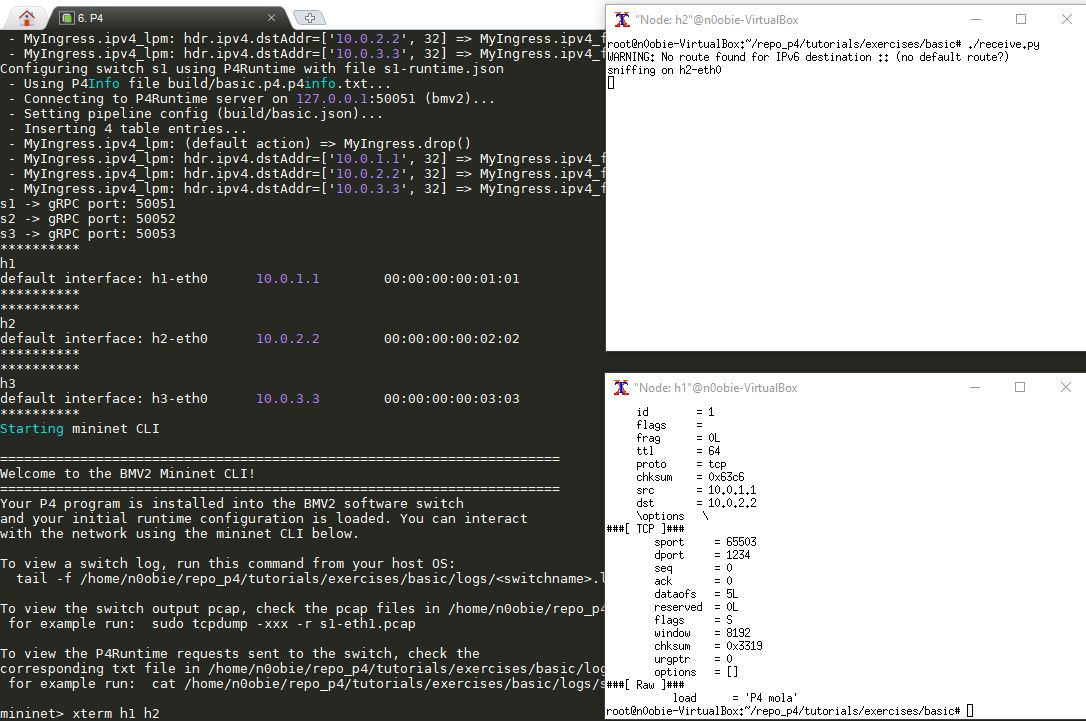
\includegraphics[width=\linewidth]{./img/test/1.JPG}
    \caption{Test Mininet: No llega el mensaje.}
  \label{fig:yo}
\end{figure}

%%%%%%%%%%%%%%%%%%%%%%%% foto terminales %%%%%%%%%%%%%%%%%%%%%%%%%

Un programa P4 define una pipe-line de procesamiento de paquetes, pero las reglas dentro de cada tabla se insertan desde el plano de control. Cuando una regla coincide con un paquete (Hay un hit), su acción se invoca con los parámetros proporcionados por el plano de control como parte de la regla.\newline
\newline
En este test, ya se ha implementado la lógica del plano de control, está suministrado por el equipo de p4. A la hora de levantar la instancia de Mininet, el comando make run instalará las reglas de procesamiento de paquetes en las tablas de cada router. Estas se definen en los archivos sX-runtime.json, donde X corresponde al número de router.\newline
\newline
Se hace uso de P4Runtime para instalar las reglas del plano de control. El contenido de los archivos sX-runtime.json se refiere a nombres específicos de tablas, claves y acciones, tal como se define en el archivo P4Info producido por el compilador (busque el archivo build / basic.p4info después de ejecutar make run). Cualquier cambio en el programa P4 que agregue o cambie el nombre de tablas, claves o acciones deberá reflejarse en estos archivos sX-runtime.json.

\subsection{Desarrollo del forwarding L3}
El archivo basic.p4 contiene un programa P4 esqueleto con piezas lógicas clave donde deberemos completar su cuerpo para el correcto funcionamiento del router. Las partes que debemos completar son las siguientes:
\begin{itemize}
    \item Completar el Parser para extraer las cabeceras de ethernet e ipv4.
    \item Completar un action llamado forward\_ipv4 que deberá: 
        \begin{itemize}
            \item Establecer el puerto de salida del paquete. 
            \item Establecer como dirección MAC origen la MAC destino de la trama recibida. 
            \item Establecer como dirección MAC destino del paquete la MAC del siguiente salto.
            \item Decrementar el campo TTL de la cabecera ipv4.
        \end{itemize}
    
    \item Completar el campo apply para decidir si aplicar la tabla.
\end{itemize}
\newpage
Para completar el parser de entrada del router hemos definido tres estados, el primer estado, entry-point, llamado start. El segundo parse\_ethernet, para extraer la cabecera de Ethernet, y decidir si si entramos a la ultima fase del parser, parse\_ipv4, en función del campo etherType. La ultima fase del parser únicamente extrae la cabecera de Ipv4. 
\begin{figure}[!htb]
  \centering
    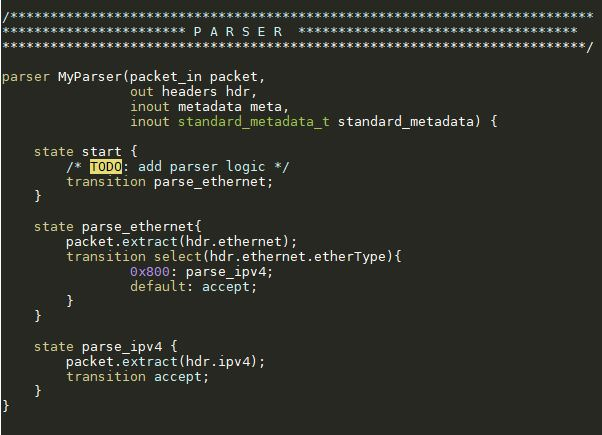
\includegraphics[width=0.8\linewidth]{./img/test/2.JPG}
    \caption{Parser.}
  \label{fig:yo}
\end{figure}
\newline
Hemos definido un action que hacer forwarding a los paquetes que les llega a los router, deberá especificar un puerto de salida, modificar las MAC para el siguiente hop, y decrementar en uno el campo TTL de la cabecera Ipv4. \newline

\begin{figure}[!htb]
  \centering
    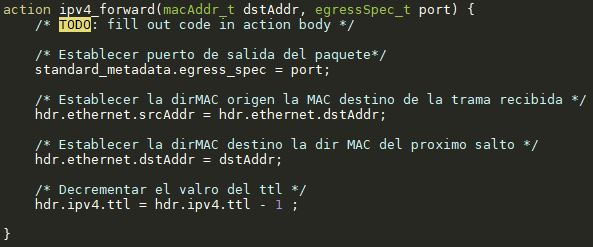
\includegraphics[width=0.8\linewidth]{./img/test/3.JPG}
    \caption{Action forwarding.}
  \label{fig:yo}
\end{figure}
Según los requerimientos dados, debemos comprobar con anterioridad si existe y es valida la cabecera Ipv4.
\newpage
\begin{figure}[!htb]
  \centering
    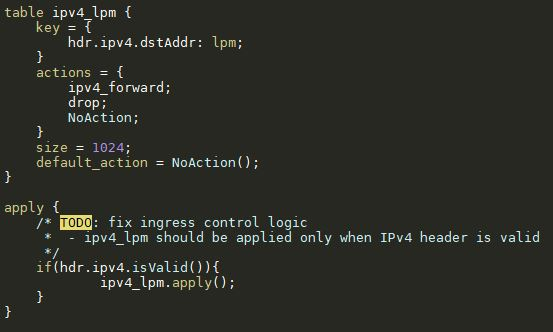
\includegraphics[width=0.7\linewidth]{./img/test/4.JPG}
    \caption{Tabla match-action de nuestro router.}
  \label{fig:yo}
\end{figure}
Por último, únicamente debemos especificar en el deparser como queremos serializar las cabeceras, y en que orden. A continuación, se incluirá la carga útil y se conformará el paquete. Por carga útil entendemos toda información no procesada por el parser de entrada por el switch p4.
\begin{figure}[!htb]
  \centering
    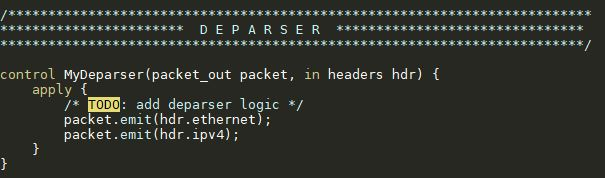
\includegraphics[width=0.8\linewidth]{./img/test/5.JPG}
    \caption{Deparser de nuestro router.}
  \label{fig:yo}
\end{figure}
\newline
\newline
A continuación, se puede apreciar en la arquitectura conformada en bloques de nuestro switch. Donde, cada bloque va especificando la funcionalidad para la que ha sido programada. Este diseño es muy útil para ver de manera la operativa funcional de nuestro switch.
\newline
\newline
\begin{figure}[!htb]
  \centering
    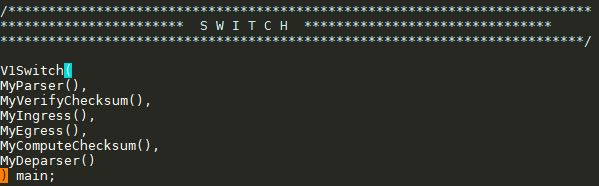
\includegraphics[width=0.8\linewidth]{./img/test/6.JPG}
    \caption{Topología funcional de nuestro switch.}
  \label{fig:yo}
\end{figure}
\newpage
A continuación, se expone como tras implementar los cambios existe conectividad en la topología entre todos los host. Para implementar los cambios antes hemos realizado un \textbf{sudo make stop} y un \textbf{sudo make clean} para limpiar los archivos residuales de los switch p4 y de Mininet.
\begin{figure}[!htb]
  \centering
    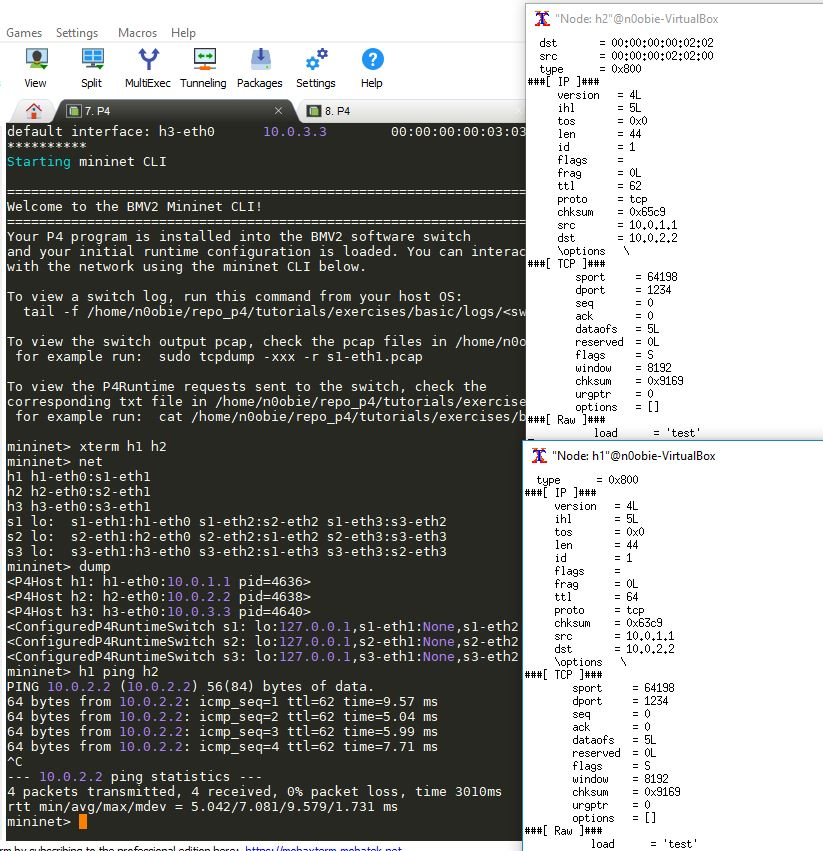
\includegraphics[width=\linewidth]{./img/test/7.JPG}
    \caption{Funcionamiento de router programado.}
  \label{fig:yo}
\end{figure}
\newpage
%%%%%%%%%%%%%%%%%%%%%%%%%%%%%%%%%%%%%%%%%%%%%%%%%%%%%%%%%%%%%%%%%%%%%%%%%%%%%%%%%%%%%%%%%%%%%%%%%%%%%%%%%%%%%%%%%%%%%%%%%%%%%%%%%%
\section{Test 2: Implementando el tunelado básico}

En este test, agregaremos soporte para un protocolo de tunelado básico al router que hicimos en el test anterior. El router básico reenvía en función de la dirección IP de destino. Tendremos que definir un nuevo tipo de encabezado para encapsular el paquete IP y modificar el código del router, para que en su lugar decida el puerto de salida utilizando una nueva cabecera de túnel.\newline
\newline
El nuevo tipo de cabecera contendrá una ID de protocolo, que indica el tipo de paquete que se está encapsulando, junto con una ID de destino que se utilizará para el enrutamiento.

\subsection{Crear protocolo de tunelado}
Siguiendo la guía debemos completar los siguientes items para conseguir el resultado del tunel entre los host.
\begin{itemize}
    \item Se debe actualizar el parser para extraer la cabecera de  myTunnel o la cabecera de  ipv4 según el campo etherType en la cabecera de  Ethernet. El etherType correspondiente al encabezado \textbf{myTunnel es 0x1212}. El parser también debe extraer el encabezado ipv4 después del encabezado myTunnel si proto\_id == TYPE\_IPV4.
    
    \item  Debemos definir una nueva acción llamada \textbf{myTunnel\_forward} que deberá situar el puerto de salida dado por el plano de control.
    
    \item Definir una tabla llamada como \textbf{myTunnel\_exact}. Esta tabla se encargará de asociar de forma exacta dado un dst\_id e invocará la acción programada anteriormente para especificar un puerto de salida idoneo para el dst\_id dado. Por defecto hará un drop.
    
    \item Hay que modificar el campo de \textbf{apply} del bloque de control de \textbf{MyIngress}. Este deberá aplicar en un primer caso la tabla \textbf{myTunnel\_exact} siempre y cuando se encuentre la cabecera myTunnel. En caso contrario se deberá aplicar la tabla del test anterior de ipv4\_lpm.
    
    \item Hay que actualizar el Deparser para que añade la cabecera nueva de myTunnel.
\end{itemize}
\begin{figure}[!htb]
  \centering
    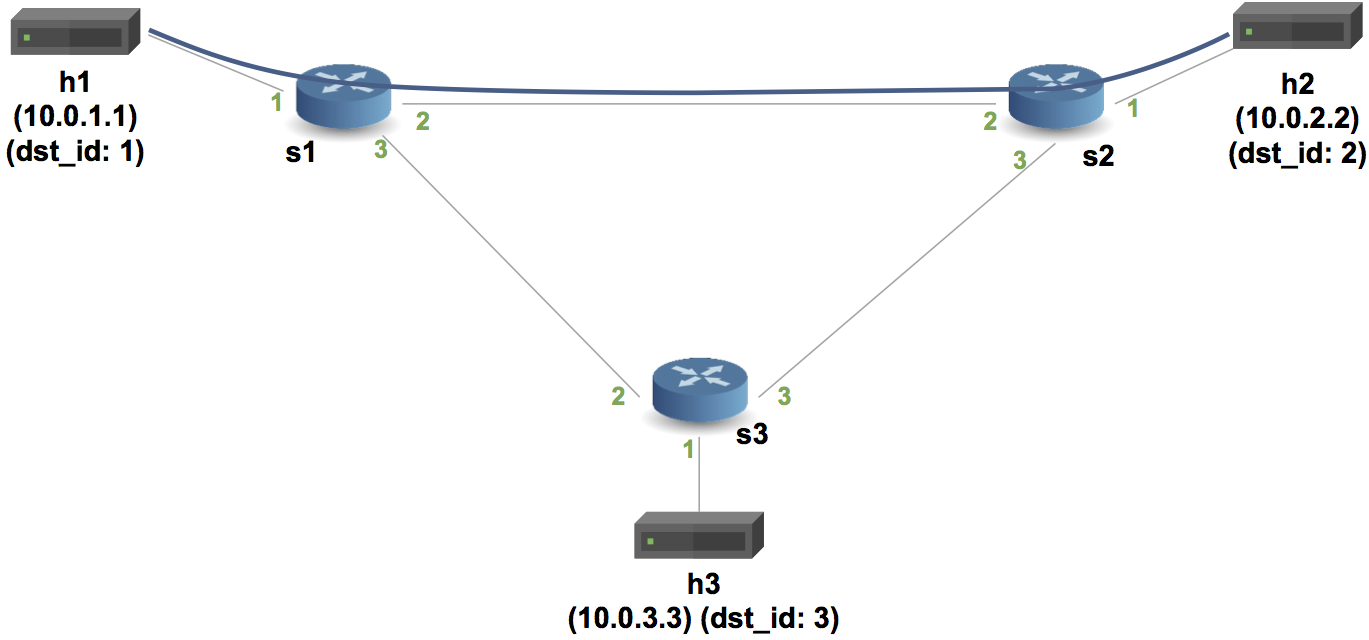
\includegraphics[width=\linewidth]{./img/test/8.png}
    \caption{Escenario a recrear.}
  \label{fig:yo}
\end{figure}
\newpage

Para cumplir el primer requerimiento se ha procedido de forma análoga al Test 1. Hemos extraído la cabecera de Ethernet, acto seguido hemos hecho un select en función del valor del EtherType, para parsearla cabecera Ipv4 o myTunnel.
\begin{figure}[!htb]
  \centering
    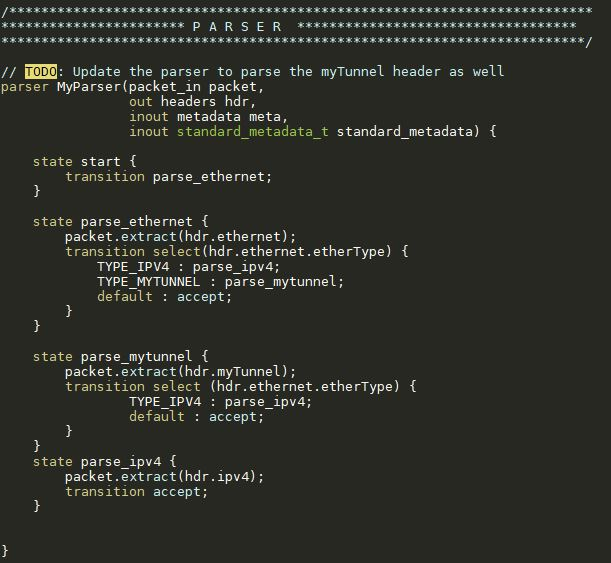
\includegraphics[width=0.7\linewidth]{./img/test/9.JPG}
    \caption{Parser actualizado.}
  \label{fig:yo}
\end{figure}

Hemos creado la nueva acción para hacer el forward hacia en puerto de salida dado por el plano de control. Esto lo especificamos indicándolo en los meta-datos asociados a ese paquete en el campo de egress port.
\begin{figure}[!htb]
  \centering
    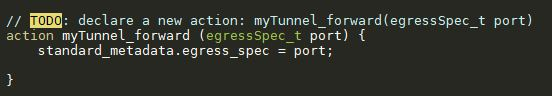
\includegraphics[width=0.7\linewidth]{./img/test/10.JPG}
    \caption{Nueva acción de forwarding.}
  \label{fig:yo}
\end{figure}
\newpage
\begin{figure}[!htb]
  \centering
    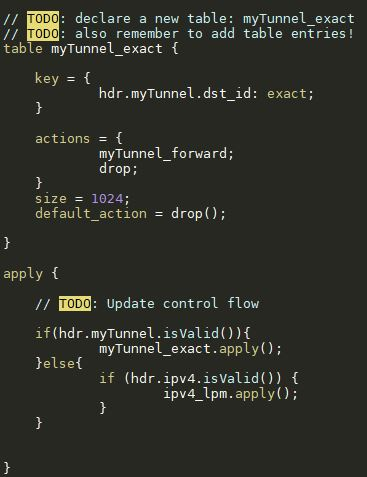
\includegraphics[width=0.5\linewidth]{./img/test/11.JPG}
    \caption{Nueva tabla de nuestro router.}
  \label{fig:yo}
\end{figure}
Para definir la nueva tabla hemos aplicado un criterio de búsqueda exacto, y que lo haga en función del dst\_id de la cabecera parseada. Si no hubiera ningún hit, por defecto se descarta el paquete. El campo  apply también ha sido actualizado para que primero se pase por la tabla de myTunnel\_exact en caso de que exista una cabecera valida de myTunnel, en caso contrario se sigu pasando por la tabla ipv4\_lpm.\newline
\newline
\begin{figure}[!htb]
  \centering
    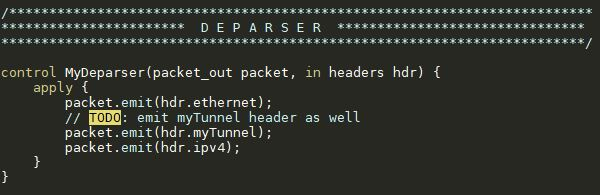
\includegraphics[width=0.8\linewidth]{./img/test/12.JPG}
    \caption{Deparser actualizado.}
  \label{fig:yo}
\end{figure}
\newline
En cuanto al Deparser únicamente se ha añadido la sentencia packet.emit(hdr.myTunnel). Esto hará que en caso de haber un paquete que contenga la cabecera myTunnel y que esta se validad, la serializará. En caso contrario omitirá esta sentencia. 
\newpage
\subsection{Parte Avanzada Tunelado}
Siguiendo la guía nos ofrecen una parte avanzada para hacer más interesante y realista del test realizado. Esto consistirá en añadir la cabecera del túnel a la entrada del túnel, y quitársela a la salida, antes de entregarle el paquete al host final. \newline
\newline
Para llevar esta tarea a cabo, nos das dos pistas que nos serán de gran utilidad.
\begin{itemize}
    \item El switch de ingreso deberá asignar en función de la dirección IP de destino el dst\_id correspondiente para el encabezado myTunnel. Además, se debe establecer el bit de validez para el encabezado myTunnel para que pueda ser emitido por el Deparser.
    \item El switch de egreso deberá eliminar el encabezado myTunnel del paquete después de buscar el puerto de salida apropiado usando el campo dst\_id.
\end{itemize}

Atendiendo a los requerimientos, a las pistas que nos han dado, hemos diseñado dos nuevas acciones que utilizaremos en el bloque de control de \textbf{MyIngress}, llamadas \textbf{myTunnel\_ingress} y \textbf{myTunnel\_egress}. Estas acciones se encargarán respectivamente de manejar la entrada y la salida del túnel. Pero, ¿Cuando sabemos que un paquete está entrando o saliendo del túnel? Una forma para saber si está entrada o al túnel hubiera sido el hecho de que el paquete no llevara cabecera myTunnel, pero cabe la posibilidad de que la IP destino del paquete sea la misma del emisor, por lo que no entraría al túnel y no sería consistente. Y lo que se complica más, saber cuando el switch es ultimo antes de salir del túnel.\newline
\newline
Si nos fijamos en el diagrama de la topología podemos apreciar como todos los switches están conectados por el puerto 1 a los host. Bingo! Para este caso nos servirá, mediante el uso de reglas estáticas (ficheros sX-runtime.json) en las tablas creadas podremos manejar los paquetes a nuestro antojo sabiendo que entran por un puerto de host y que no llevan cabecera myTunnel, se la añadiremos. También cuando el valor del dst\_id sea el correspondiente al host que tiene más próximo a el le quitaremos la cabecera del túnel ya que ya a llegado a su destino, y lo sacamos por el puerto 1.
\newline
\begin{figure}[!htb]
  \centering
    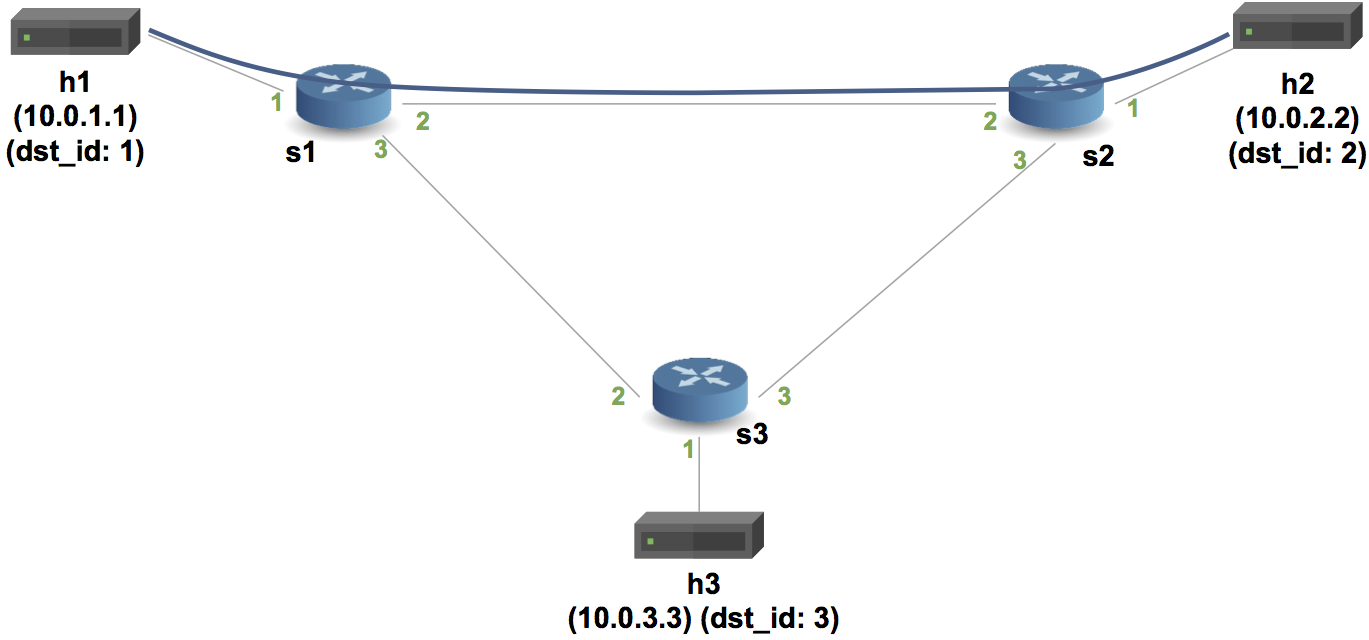
\includegraphics[width=\linewidth]{./img/test/8.png}
    \caption{Escenario.}
  \label{fig:yo}
\end{figure}
\newline
En este caso nos favorece la disposición del escenario, pero en caso contrario habría que darle más complejidad al procesado de paquetes. Sabiendo ya la estrategia a implementar, se dota de funcionalidad las acciones anteriormente descritas. 
\newpage
Como se puede apreciar en la acción myTunnel\_ingress nos encargaremos, de establecer un puerto de salida apropiado (forwarding), marcar la cabecera como validad, guardar en el campo proto\_id de la cabecera myTunnel el protocolo superior que va sobre él (Copiamos el valor que tenía el etherType antes), indicar en la trama de Ethernet el campo etherType, que el protocolo superior es myTunnel, y por último establecer un dst\_id dado por el plano de control.
%%%%%%%%%%%%%%%%%%%%%%%%%%%%%%%%%%%%%%%%%%%%%%%%%%%%%%%%%%%%%%%%%%%%%%%%%%%%%%%%
\begin{figure}[!htb]
  \centering
    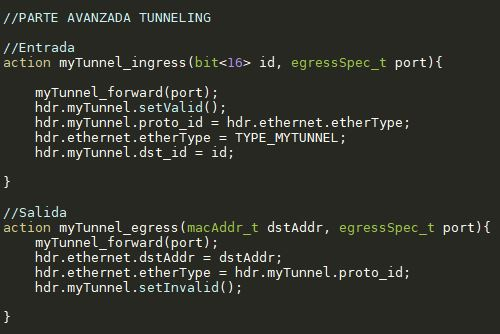
\includegraphics[width=0.8\linewidth]{./img/test/13.JPG}
    \caption{Acciones myTunnel\_ingress y myTunnel\_egress.}
  \label{fig:yo}
\end{figure}
%%%%%%%%%%%%%%%%%%%%%%%%%%%%%%%%%%%%%%%%%%%%%%%%%%%%%%%%%%%%%%%%%%%%%%%%%%%%%%%%
\newline
En cuanto a la acción myTunnel\_egress, se encargará de hacer forwarding de la cabecera myTunnel, modificar las cabeceras de Ethernet para establecer el destino y modificar el etherType con el valor del proto\_id. Además, invalidamos la cabecera myTunnel para sacarla del paquete a la hora de hacer el des-parseo.\newline
\newline
De forma adicional, hemos tenido que añadir estas dos nuevas acciones a las tablas ya creadas. Para así poder hacer uso de ellas cuando se estime oportuno.
\begin{itemize}
    \item  ipv4\_lpm
    \item  myTunnel\_exact
\end{itemize}
Con la tabla ipv4\_lpm controlaremos el acceso al túnel y con la tabla myTunnel\_exact controlaremos la salida al túnel.
\newpage
\begin{figure}[!htb]
  \centering
    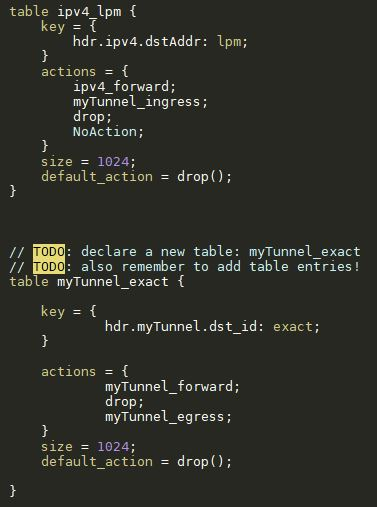
\includegraphics[width=0.5\linewidth]{./img/test/14.JPG}
    \caption{Tablas actualizadas.}
  \label{fig:yo}
\end{figure}
La lógica que se ha seguido para aplicar estas tablas ha sido la siguiente, si la cabecera Ipv4 es valida y la cabecera de myTunnel es invalida ( o no está presente), aplicamos la tabla ipv4\_lpm. En caso contrario, la cabecera myTunnel será valida, por lo que aplicaremos la tabla de myTunnel\_exact para poder gestionar la salidas del túnel.\newline
\newline
\begin{figure}[!htb]
  \centering
    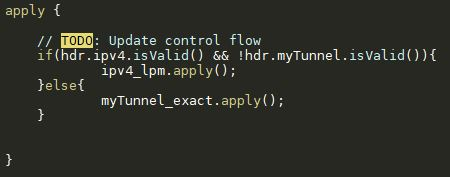
\includegraphics[width=0.7\linewidth]{./img/test/15.JPG}
    \caption{Lógica para aplicar las tablas.}
  \label{fig:yo}
\end{figure}
\newpage
Por último, solo quedaría definir como van a ser las entradas de las tablas ipv4\_lpm y myTunnel\_exact . Al igual que en el test de tunelado básico, las entradas serán estáticas. Estarán definidas por archivos json, cada switch tendrá su fichero con las distintas entradas que regirán cada tabla de cada switch. Por así decirlo, estos ficheros actuaran como la parte de control de nuestra topología. \newline
\newline
\begin{figure}[!htb]
  \centering
    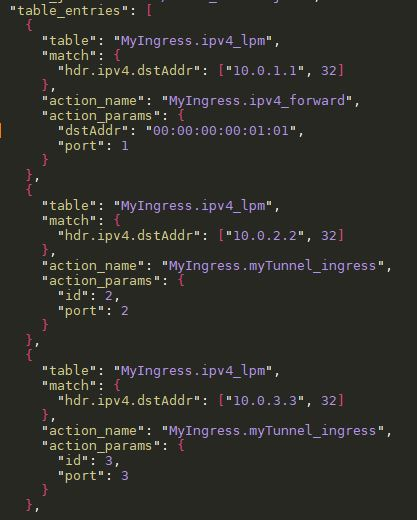
\includegraphics[width=0.7\linewidth]{./img/test/16.JPG}
    \caption{Definición de entradas a las tablas del switch 1.}
  \label{fig:yo}
\end{figure}
\newline
Se puede apreciar como cada entrada tiene definidos un match y una acción. De forma adicional, en el caso de que la acción lo requiera se deberá suministrarle los parámetros apropiados. Por ejemplo en tabla que gestionará la entrada del switch 1, aplicaremos la acción de myTunnel\_ingress siempre y cuando el paquete tenga como destino IPv4 distintas al host 1 que tiene directamente conectado al switch. \newline
\newline
En función, de la dirección destino ipv4, deberemos pasarle unos parámetros adecuados a la acción myTunnel\_ingress, identificador de tunel y el puerto por el cual el switch debe sacar el paquete. De esta manera se procedería de forma análoga, en la tabla myTunnel\_exact y en los otros switch, adecuando y corrigiendo las entradas para conseguir la funcionalidad deseada.  
A continuación, dejamos dos grafos describen la operativa funcional de los switches programados en este test. Los grafos harán referencia a los dos bloques más simbólicos del switch, el MyParser y MyIngress donde se lleva a cabo la lógica del switch. 
\newpage
\begin{figure}[!htb]
  \centering
    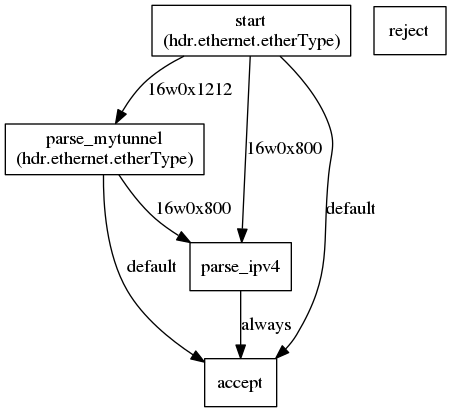
\includegraphics[width=0.7\linewidth]{./img/test/17.png}
    \caption{Bloque funcional MyParser}
  \label{fig:yo}
\end{figure}
\begin{figure}[!htb]
  \centering
    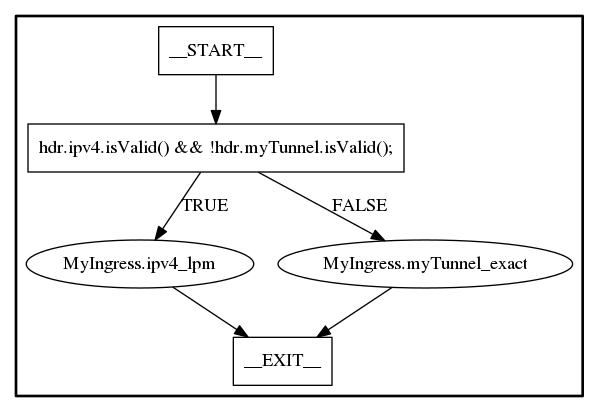
\includegraphics[width=0.7\linewidth]{./img/test/18.png}
    \caption{Bloque funcional MyIngress}
  \label{fig:yo}
\end{figure}
Más información de como generar estos grafos a partir de programas p4 en el \hyperref[chap:como generar grafos desde programas p4]{\textit{apartado B de los anexos}}. 
\newpage
\section{Test 3: Implementación del plano de control vía P4Runtime}
En este test, se va a usar P4Runtime para enviar entradas a las tablas del switch en lugar de utilizar la CLI del switch. El programa es el mismo programa P4 que se utilizó en la parte avanzada de tunneling. De forma adicional se han añadido dos contadores (\textbf{ingressTunnelCounter}, \textbf{egressTunnelCounter}). Se utilizarán para llevar la contabilidad de paquetes procesados.\newline
\newline
Para implementar el plano de control se hará uso del script \textbf{mycontroller.py}, y algunas bibliotecas auxiliares en el directorio p4runtime\_lib para crear las entradas de la tabla necesarias para encaminar el tráfico entre el host 1 y 2.

\subsection{Escenario previo}

El código para esta asignación de entradas a las tablas de los switch se encuentra en un archivo llamado \textbf{mycontroller.py}, y solo instalará algunas de las reglas que necesita para canalizar el tráfico entre dos hosts (h1, h2). \newline
\newline
Si compilamos el programa p4 y lanzamos Mininet podremos comprobar como  no hay conectividad entre los host, eso se debe a que los paquetes que le llegan pase la fase de parseo, pero cuando llegan a la fase MyIngress, y ya han pasado por la acción de myTunnel\_ingress, al no haber entradas en la tabla myTunnel\_exact correspondientes al forwarding de los paquetes que ya tienen cabecera myTunnel, estos no consiguen salir por el puerto correspondiente y alcanzar al siguiente switch, ya que por defecto la acción instalada es dropear los paquetes.\newline
\newline

